%!TEX program = xelatex
% 完整编译: xelatex -> biber/bibtex -> xelatex -> xelatex
\documentclass[lang=cn,11pt,a4paper]{elegantpaper}

\title{嘟嘟收件箱——基于Web应用的作业收集利器}
%\author{华中科技大学\ \ 张庙松 \ \ 张隽翊 \ \ 赵宇航}
\institute{}

\version{1.0}
\date{\zhtoday}


% 本文档命令
\usepackage{array}
\usepackage{listings}

% 导入包
\usepackage{hyperref}
\usepackage{color,soul}
\usepackage{ctex}
\usepackage{xeCJK}
\usepackage{xcolor}
\setCJKmainfont{SimSun} % 设置中文字体
\newcommand{\hlc}[2][yellow]{\colorbox{#1}{#2}} % 定义一个高亮命令
% 格式设置
\hypersetup{hidelinks,
	colorlinks=true,
	allcolors=blue,
	pdfstartview=Fit,
	breaklinks=true}
\newcommand{\ccr}[1]{\makecell{{\color{#1}\rule{1cm}{1cm}}}}

\begin{document}

\maketitle
\thispagestyle{empty} % 将当前页的页眉和页脚样式设置为空
\begin{abstract}
本文为嘟嘟收件箱软件的说明文档,它是一款基于计算机Web技术的免费开源解决方案,旨在满足学生群体的个性化和集中式需求。该软件可以将学生从繁琐耗时的无意义活动中解放出来,提高学生的效率和学习体验。通过本文的介绍,您可以深入了解嘟嘟收件箱软件的功能和优势,并了解如何使用该软件来管理作业收集。
\keywords{学习,工作,作业收集,效率,Web软件应用}
\end{abstract}
\clearpage % 确保分页
\tableofcontents
\thispagestyle{empty} % 将当前页的页眉和页脚样式设置为空
\clearpage % 确保分页
\pagenumbering{arabic} % 从 1 开始计数页码
\setcounter{page}{1} % 将页码计数器设置为 1
\section{需求分析}
\subsection{背景}
在现行的教学模式下,教师通常会要求学生通过电子版或者压缩包的方式提交作业,并由班长或学委进行统计收集,学委需要对每一个人的提交进行管理,非常繁琐且耗费时间。随着互联网和移动设备的普及,基于Web应用的作业收集和批改软件开始逐渐出现,提供了更加高效的作业管理方式。


\subsection{目标用户}
嘟嘟收件箱软件旨在为学生提供一个方便、集中的工具,以帮助他们更好地组织和管理他们的学习任务,其目标用户如下:
\begin{itemize}
    \item 班长、学委等需要进行作业收集工作的班干部
    \item 直接进行作业收集的助教
    \item 其他需要集中式收集解决方案的集体
\end{itemize}

\subsection{竞品分析}
目前市场主流的拥有作业收集功能的应用以腾讯文档为例,目前市场上的同类应用有如下的缺点:
\begin{itemize}
	\item 卡顿和加载慢的问题:应用是基于云技术实现的,它需要通过网络连接访问远程服务器,因此在网络状况不佳或者访问量较大的情况下,可能会出现卡顿和加载慢的问题。这些问题可能会对用户的使用体验造成不便和影响。
	
	\item 功能相对简单:目前市场上的软件应用的功能相对简单,缺乏一些高级功能,如批量化重命名,直观性数据分析统计,复杂环境下的应用使用等。
	
	\item  对PC端支持不够完善:现有的轻量级作业收集应用大多集中于移动端的使用,虽然一定程度上满足了移动性的需求,但是移动端的编辑和格式调整功能较为有限,无法完全满足需求。此外,由于移动设备的屏幕较小,使用应用进行文档编辑时可能会出现一些不便,影响用户的使用体验。
	\item 隐私问题引发担忧:现有的作业收集应用使用时,无论管理员还是普通用户,都需要提供个人的身份信息,引发了关于个人信息泄露的隐私问题的担忧。
	\item 缺乏个性化定制功能:应用缺乏一些个性化定制功能,如自定义快捷键和一键催交等。这些功能可以帮助用户更好地使用,提高工作效率,目前的主流应用鲜有提供这些功能。
\end{itemize}






\clearpage
\section{概要设计}


\subsection{总体设计}


\subsection{项目模块功能设计}

\clearpage
\section{详细设计}


\subsection{界面设计}

\subsubsection{普通用户界面设计}

\subsubsection{管理用户界面设计}

\subsection{数据库技术}

\subsection{关键技术}

\clearpage

\section{测试报告}
\subsection{测试目的和范围}
本次测试的目的是验证应用程序的完整性和各个功能的正确性。测试范围包括应用程序的后端构建和自动化单元测试。

\subsection{测试方法和工具}
我们使用了Flask提供的测试客户端和Python标准库内置的unittest框架进行自动化单元测试。测试客户端模拟了一个Web服务器环境,可以通过 get()和 post()方法模拟客户端对服务器发送请求,并获取响应数据。unittest框架自动识别test\_*模式的文件,可以方便地进行单元测试。

接下来,我们将介绍测试的过程、测试用例设计、测试结果以及分析等内容,以及对应用程序的性能和质量进行评估和总结,并提出后续改进和优化的建议。
\subsection{测试环境}
\begin{itemize}
	\item 开发环境:Windows 10 \& 11 + Deepin Linux v20.7.1
	\item 运行环境:Ubuntu 20.04 LTS Server on Aliyun ECS
	\item 编程语言:Python 3.7+
	\item 程序框架:
		\begin{itemize}
			\item 前端:React框架和Ant Design组件
			\item 后端:SQLAlchemy in Python
		\end{itemize}
	\item IDE:PyCharm Professional + Visual Studio Code
	\item 实现语言:Python + HTML5 + CSS3 + JavaScript
\end{itemize}

\subsection{程序测试}
\clearpage
\section{使用指南}

我们已将应用程序部署到互联网上,您可以访问我们的网站{\href{http://writebug.pythonanywhere.com/}{嘟嘟收件箱}}以使用它。在下面的内容中,我们将从不同类型的用户的角度介绍如何使用应用程序。相关的使用指南我们也部署到了互联网上,你可以通过访问{\href{https://slapaf.github.io/HUST-SE-2022/}{嘟嘟收件箱使用指南}}来获得在线指南。

我们将用户分成两类:收集者和提交者。其中,收集者是指创建提交任务的用户,例如老师或班委;提交者是指提交作业的用户,例如普通学生。

以下是每个用户类型的指南:

\subsection{收集者}
\begin{itemize}
	\item {\bf 注册}\\
	如果您之前没有在我们的网站使用过,需要先进行注册。具体步骤如下:
	\begin{enumerate}[label=\arabic*)]
		\item 打开嘟嘟可收件箱Web端网页。
		\item 点击\hlc{注册}进入注册页面。
		\item 填写用户名、密码等相关信息,包括必填项用户名、密码、邮箱。
		\item 注册成功后再登录使用。如下图所示:
		\begin{figure}[!htb]
			\centering
			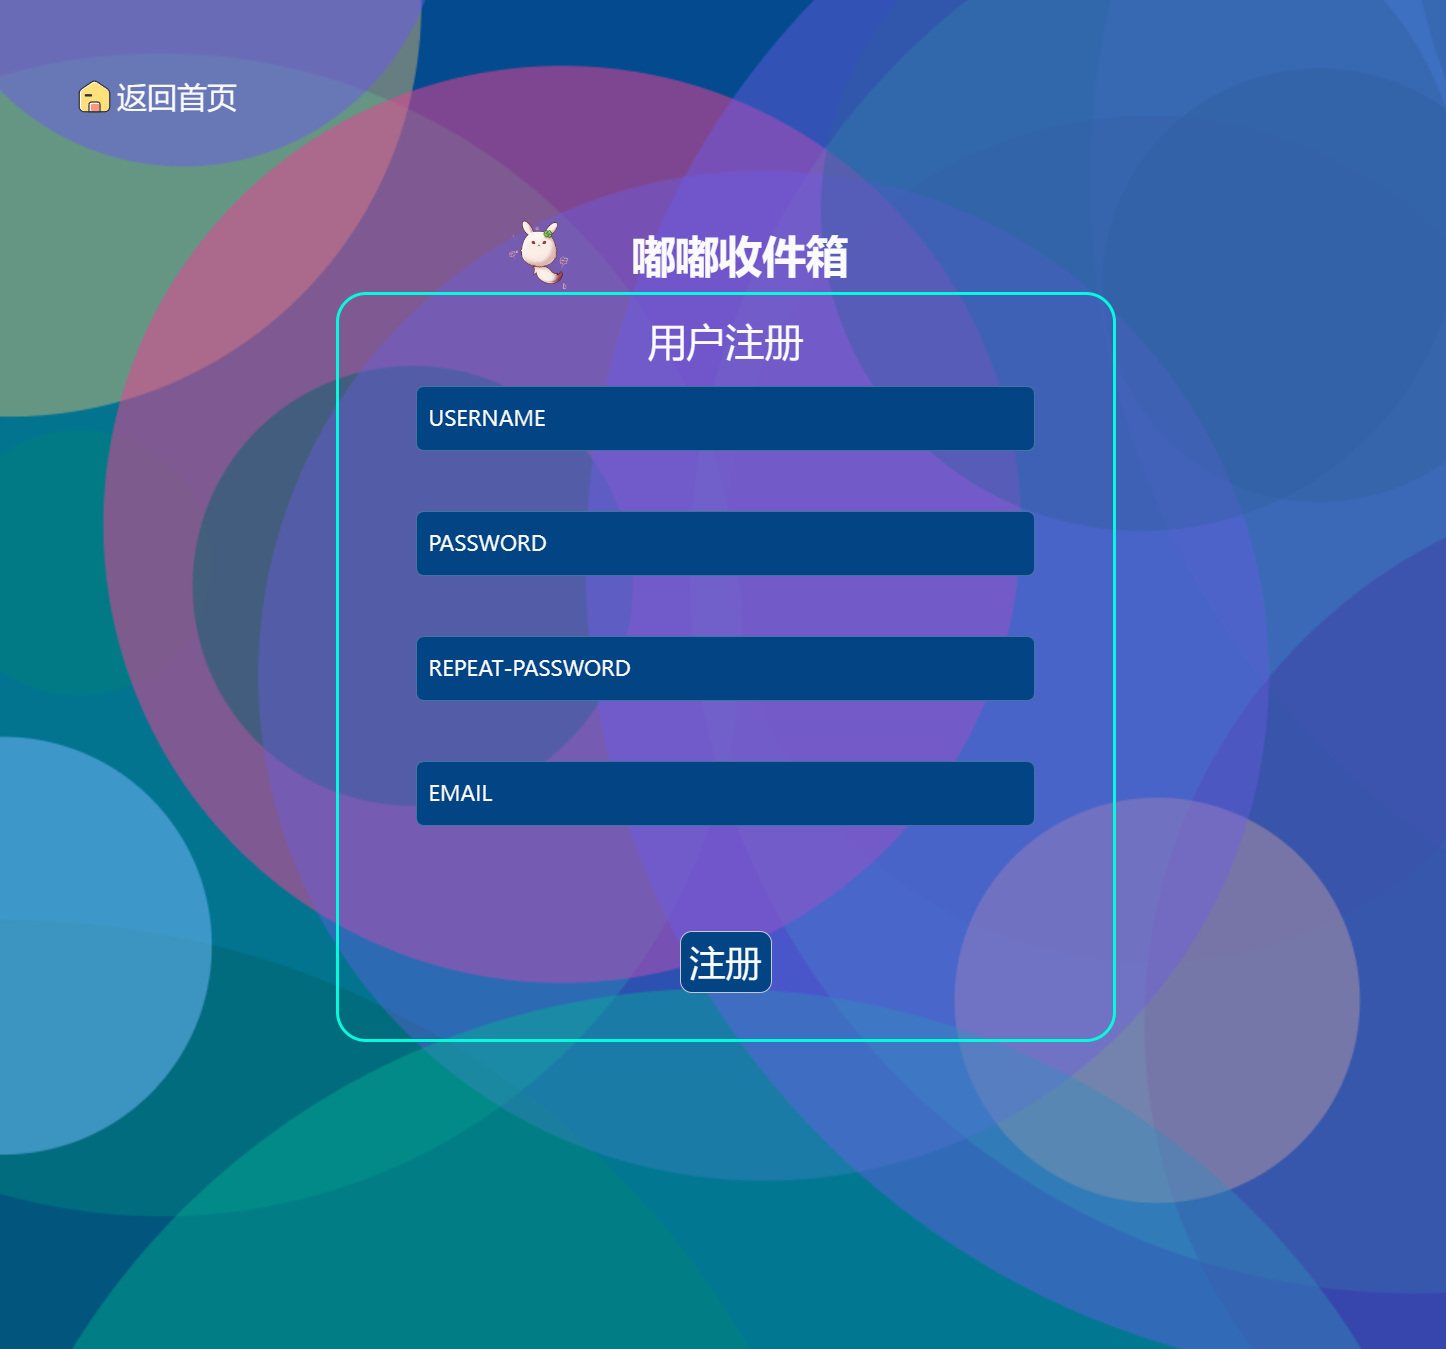
\includegraphics[width=0.9\textwidth]{注册.png}
		\end{figure}
	
	
		{\bf Tips:请注意,在您注册的过程中,包括用户名,密码,邮箱字段为必填项。}
	\end{enumerate}
	\item {\bf 登录}
	
	如果您已经成功注册,可以在我们的网页上点击\hlc{登录}进入登录页面。填写注册帐号的用户名、密码,点击登录按钮即可使用。如下图所示:
	\begin{figure}[!htb]
		\centering
		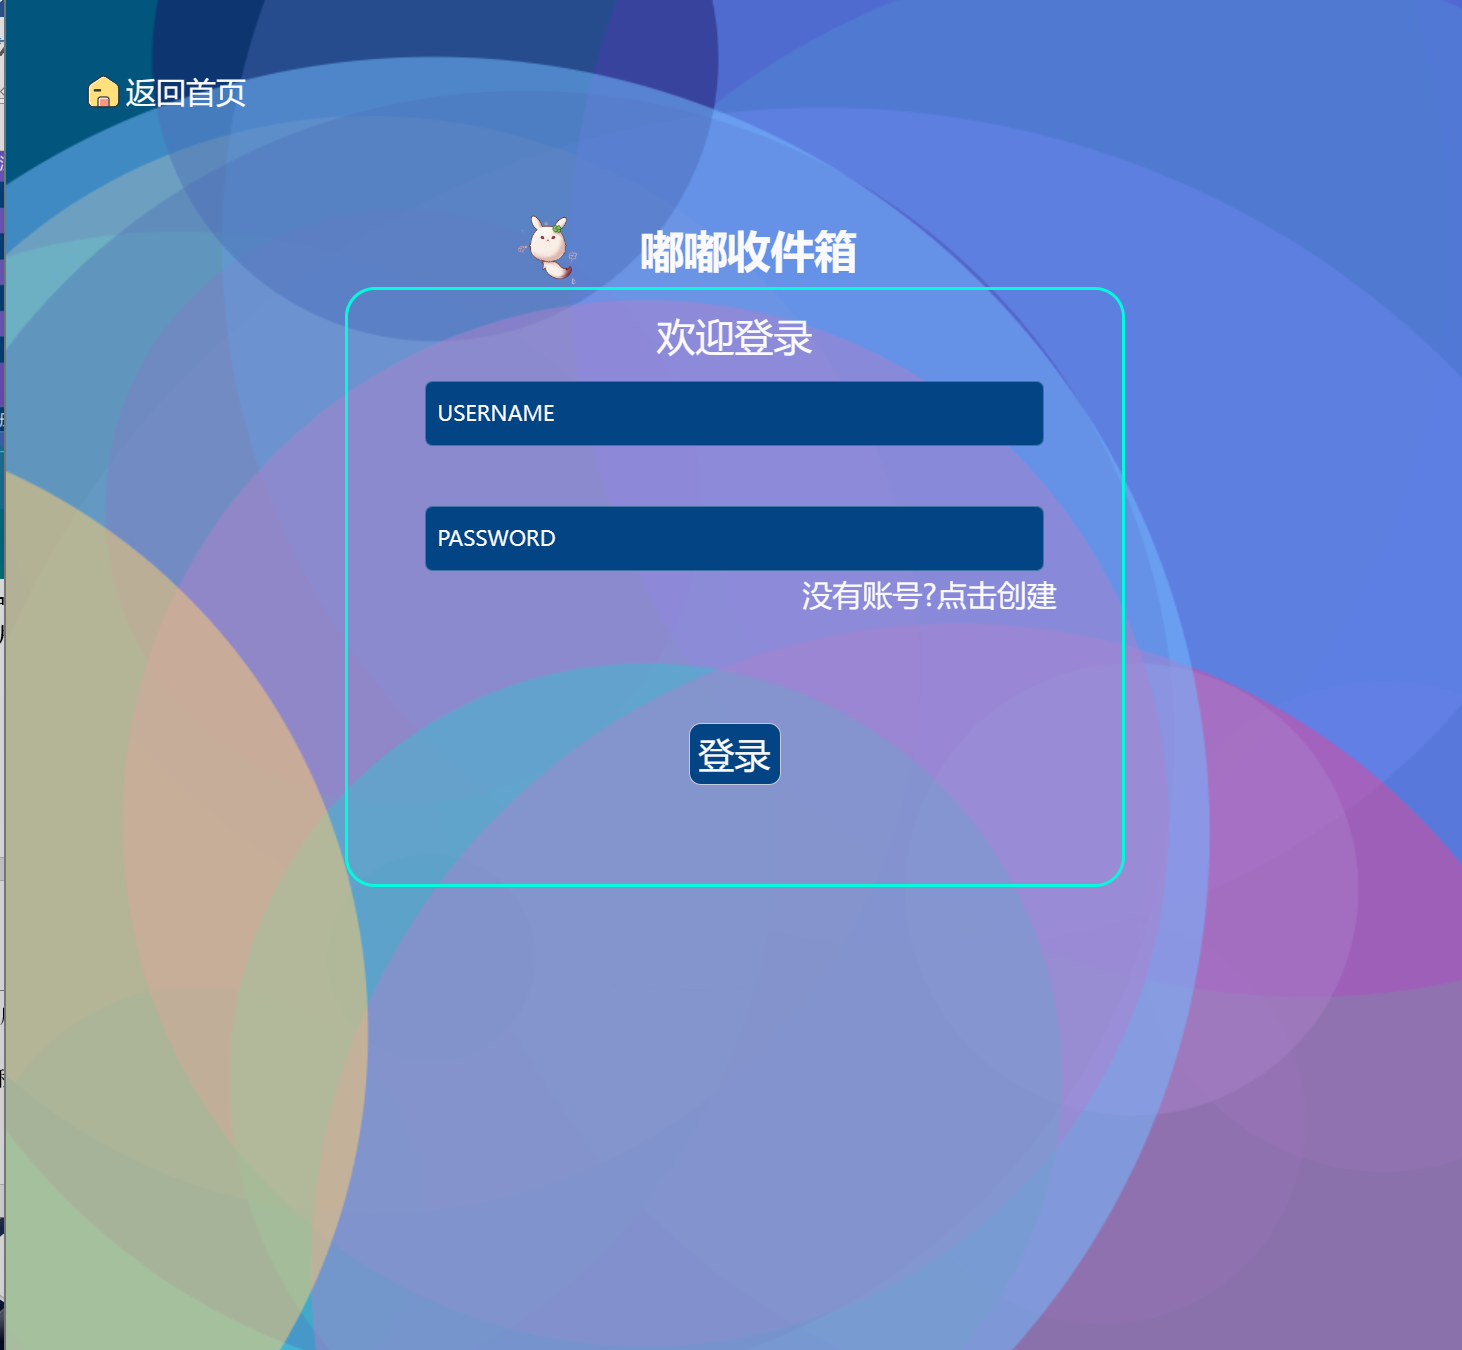
\includegraphics[width=0.9\textwidth]{登录.png}
	\end{figure}
	\item {\bf 创建收集}
	
	在成功登录后,点击\hlc{创建收集}{\bf }按钮,进入创建收集界面。需要设置的信息大致包括收集标题、收集者、截止时间、详情描述以及具体的题目。
	
	创建收集的页面如下图所示,系统默认添加了简答题,单选题,多选题,文件收集题共四个题目:
	\clearpage
	\begin{figure}[!htb]
		\centering
		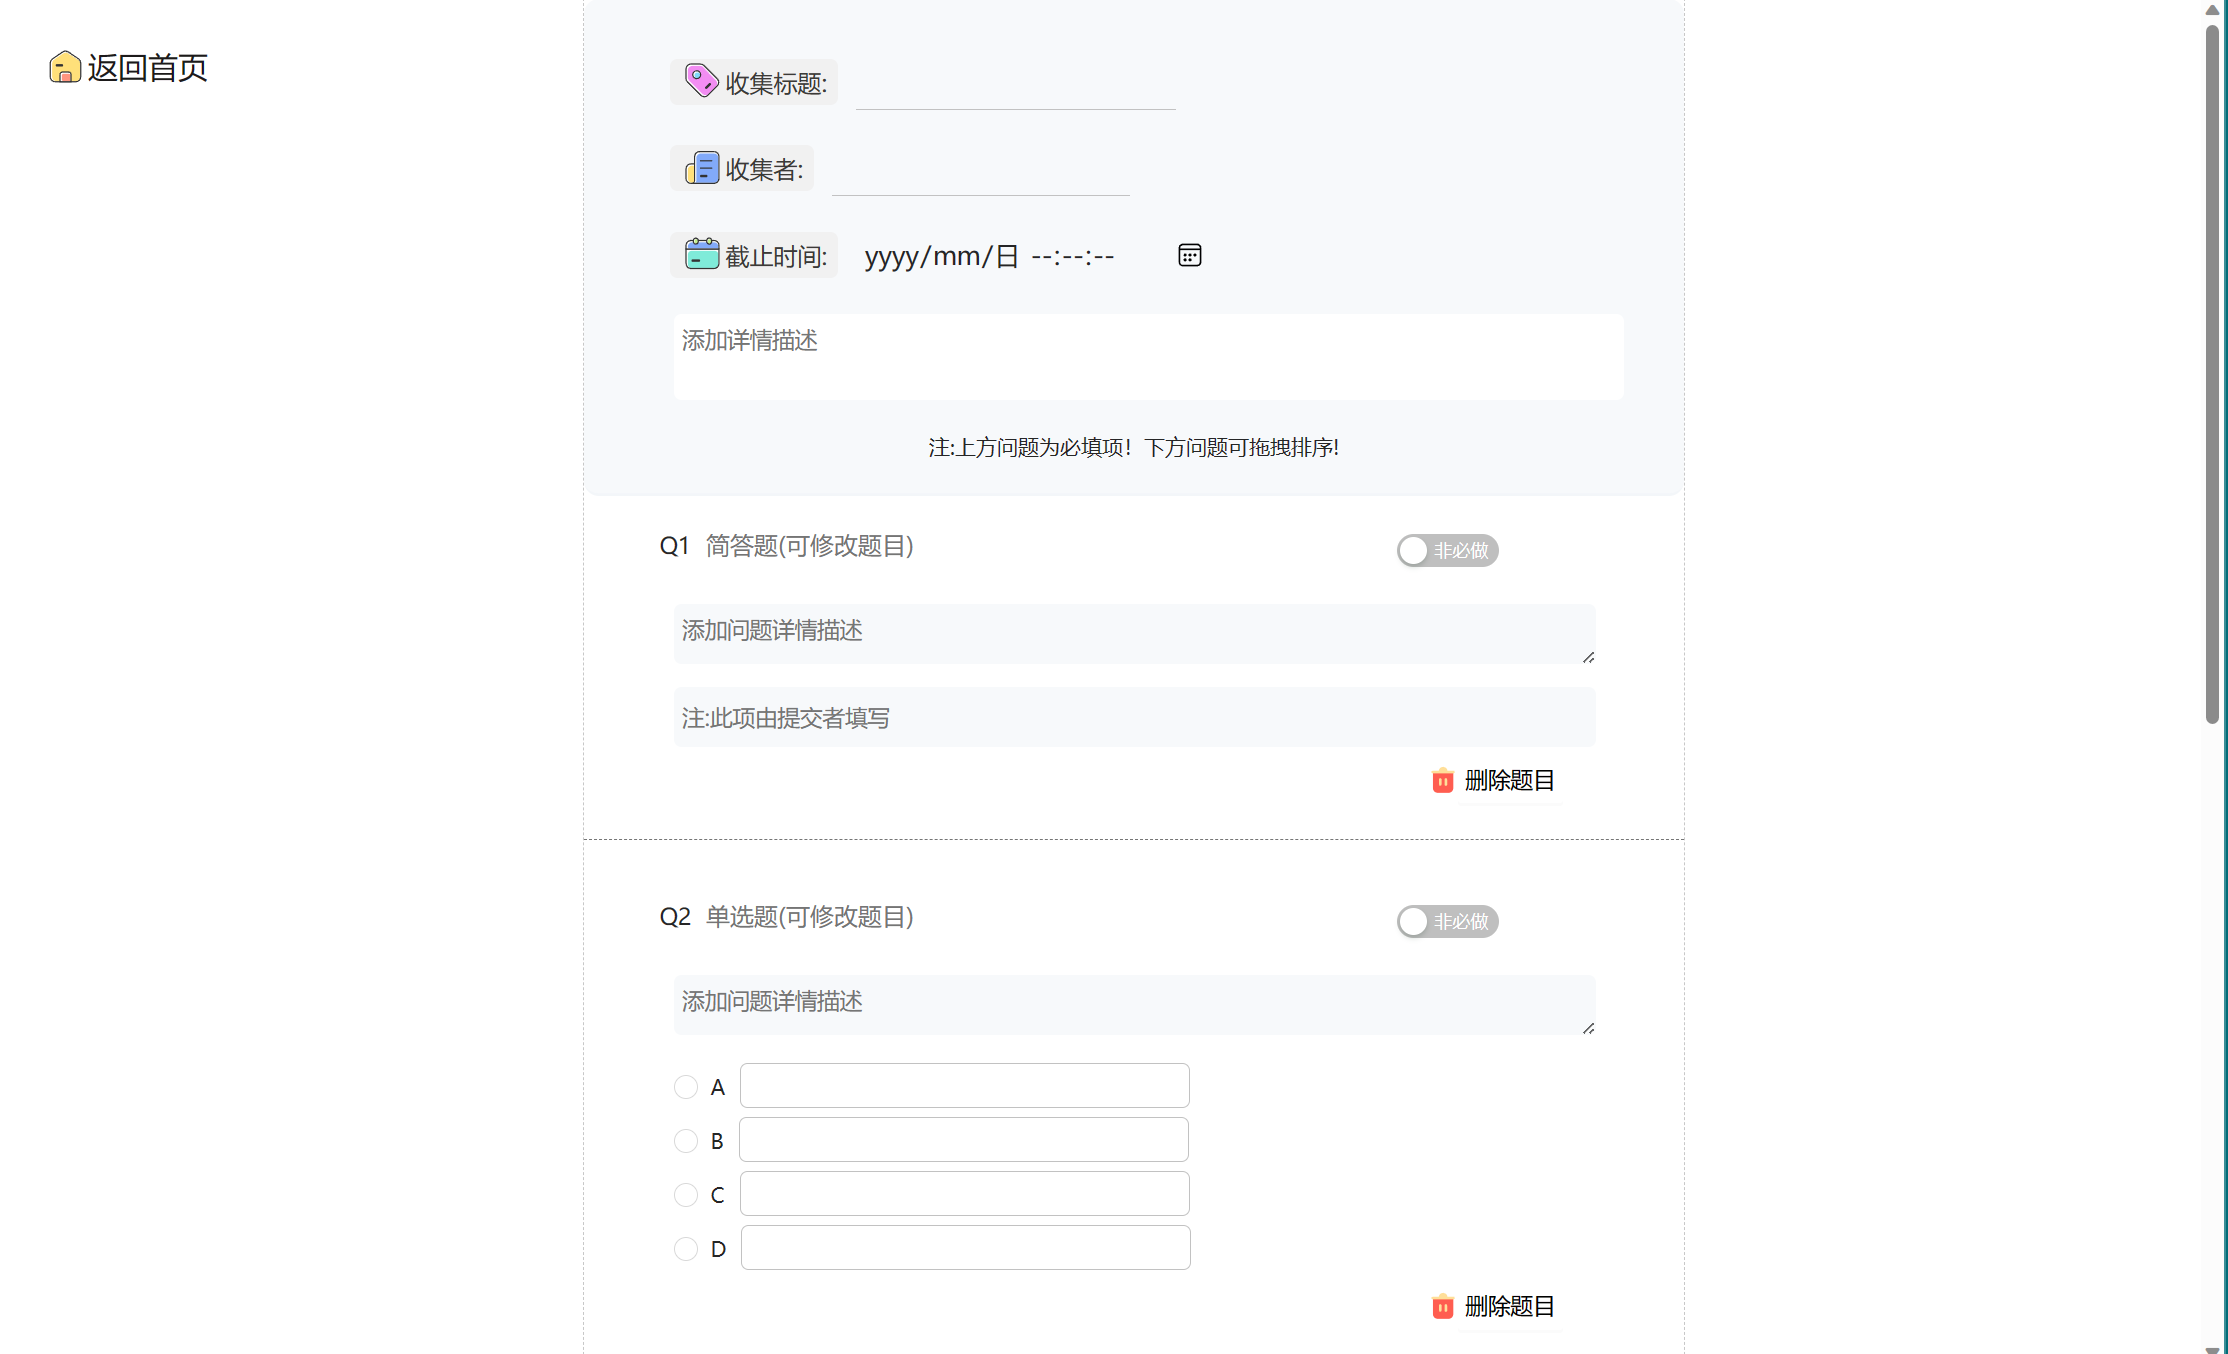
\includegraphics[width=0.9\textwidth]{创建收集1.png}
	\end{figure}
	\begin{figure}[!htb]
	\centering
	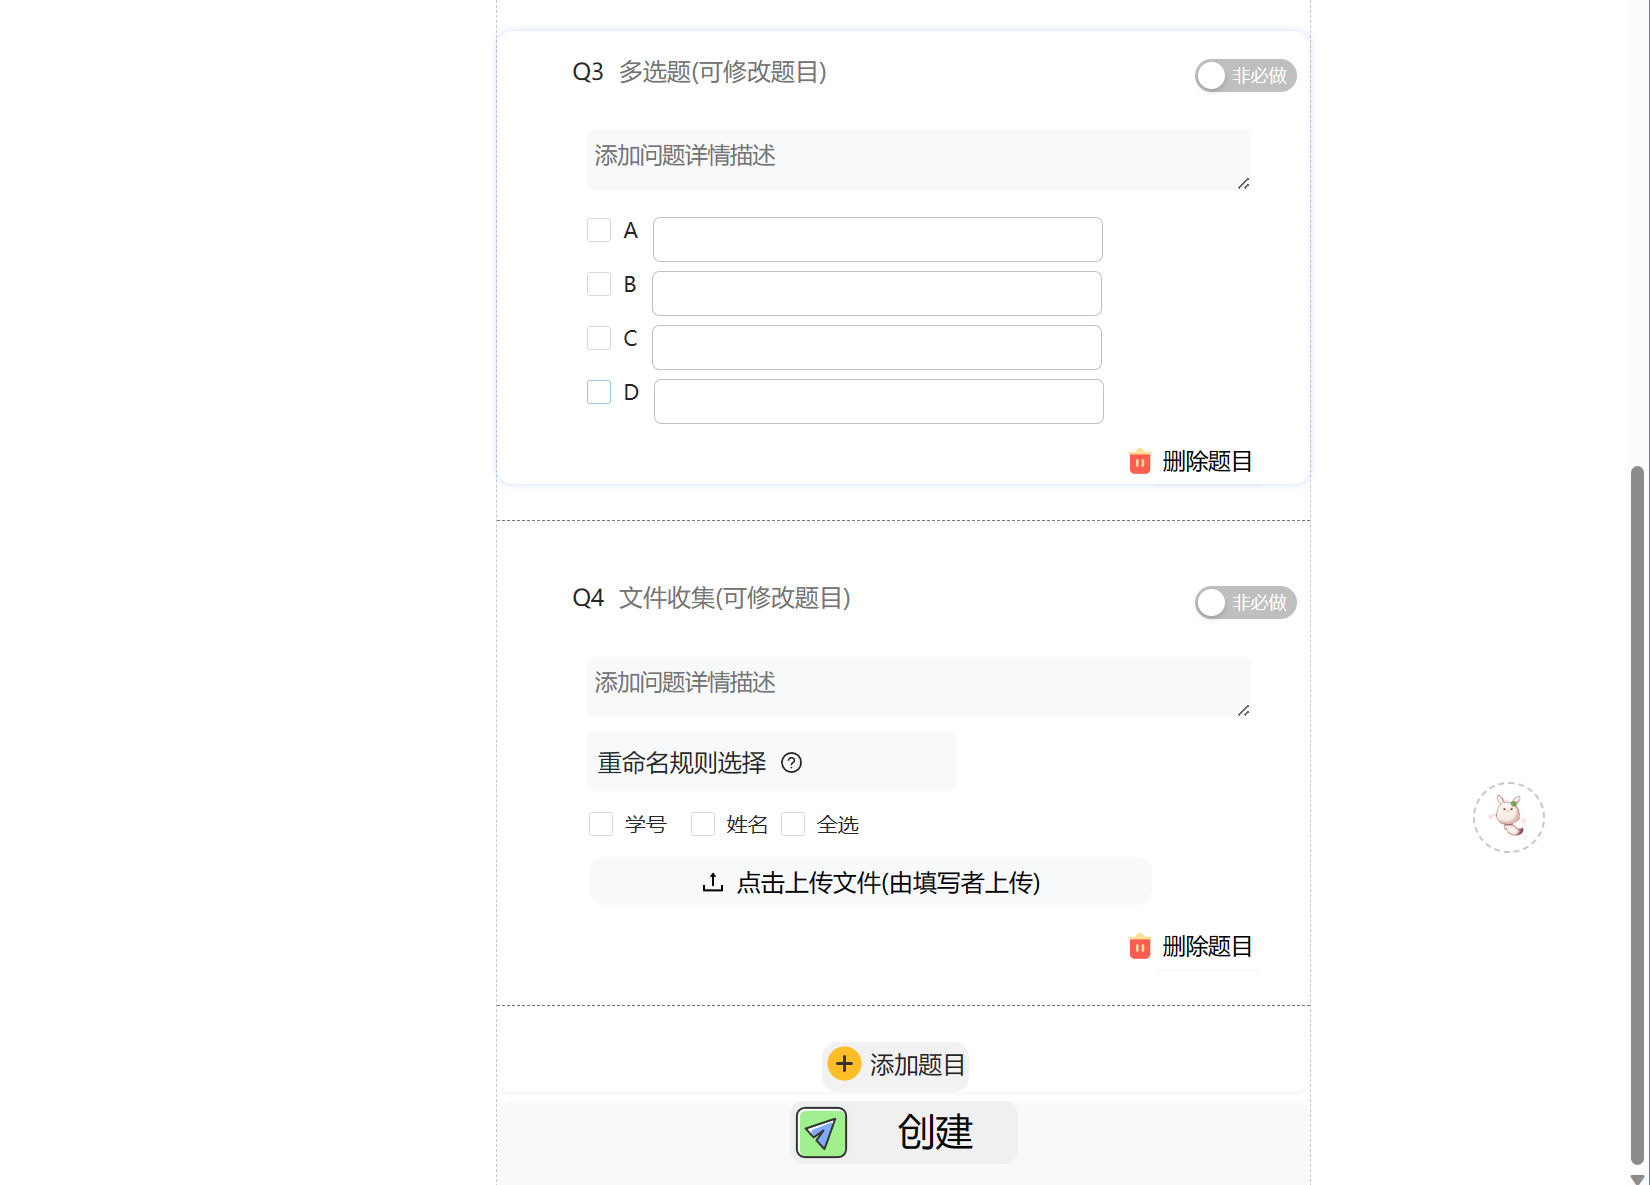
\includegraphics[width=0.9\textwidth]{创建收集2.png}
\end{figure}
	具体内容如下:
	
	\begin{itemize}
		\item {\bf 收集标题:}设置收集的名称,默认为“文件收集”。
		\item {\bf 收集者:}设置收集者。用于提交者鉴别创建收集的人员和信息提交渠道,防止信息泄漏。
		\item {\bf 截止时间:}设置收集的截止时间。在截止日期之前的提交视为有效提交,截止日期之后该收集状态会由进行中转为已截止。\\
		{\bf Warning: 截止时间不得早于当前时间,否则将无法创建收集。}
		\item {\bf 详情描述:}设置收集的相关描述信息。如向提交者提供相关说明,交待各个题目的提交格式等。
		\item {\bf 具体题目:}收集问卷中可以创建多种类型的题目,包括填空题、选择题、文件题和问卷题。
		\begin{enumerate}
			\item {\bf 填空题}:需要设置题目名称、详情描述这两项信息。在收集发布后,提交者在下方的文本框内填写信息。
			\item {\bf 选择题}:选择题分为单选题和多选题两种类型。
			\begin{itemize}
				\item {\bf 单选题}:需要设置题目名称、详情描述和正确选项,选项信息需要在详情描述中给出。点击正确选项前的圆形框,变为实心代表选中该项。单选题只能设置 1 个正确选项,最多设置 4 个可选项。
				\item {\bf 多选题}:需要设置题目名称、详情描述和正确选项,选项信息需要在详情描述中给出。点击正确选项前的圆形框,变为实心代表选中该项。多选题需要设置至少 2 个正确选项,最多设置 4 个可选项。
			\end{itemize}
			\item {\bf 文件题}:需要设置题目名称、详情描述,可以设置重命名规则。\
			{\bf 重命名规则}用于统一提交者上传的文件命名,方便整理。命名规则来自于问卷中其他填空题的题目名称,最终收集到的文件会按照形如“题目1 + 题目2”的格式进行重命名。
		\end{enumerate}
		所有题目的右下角有\hlc{删除题目}按钮,点击可以去掉对应的题目。题目支持拖拽排序,可以通过鼠标按住拖动的方式设置题目在问卷上的排列顺序。\\
		{\bf Info: 拖拽排序识别比较严格,需要被拖动的题目覆盖待放置位置的题目所在区域才可执行。}
	{\bf Tips:创建收集时,收集标题、收集者、截止时间为必填项。	}
	\end{itemize}
	\item {\bf 发布收集}\\
	编辑完毕后,点击最下方的\hlc{创建}按钮,如果所有必填项都设置正确就能创建收集,否则系统会提示哪些项目是必须填写的,修改正确后才能创建。创建完毕的收集会生成一个收集链接,通过点击\hlc{分享}按钮可以将收集链接发送给提交者进行提交。\
	\item {\bf 查看收集}\\
	创建好的收集会在“我的收集”页面中显示,您可以点击\hlc{收集记录}按钮进入该页面,根据收集标题等相关信息快速查找所需要的收集。
	\clearpage
		\begin{figure}[!htb]
		\centering
		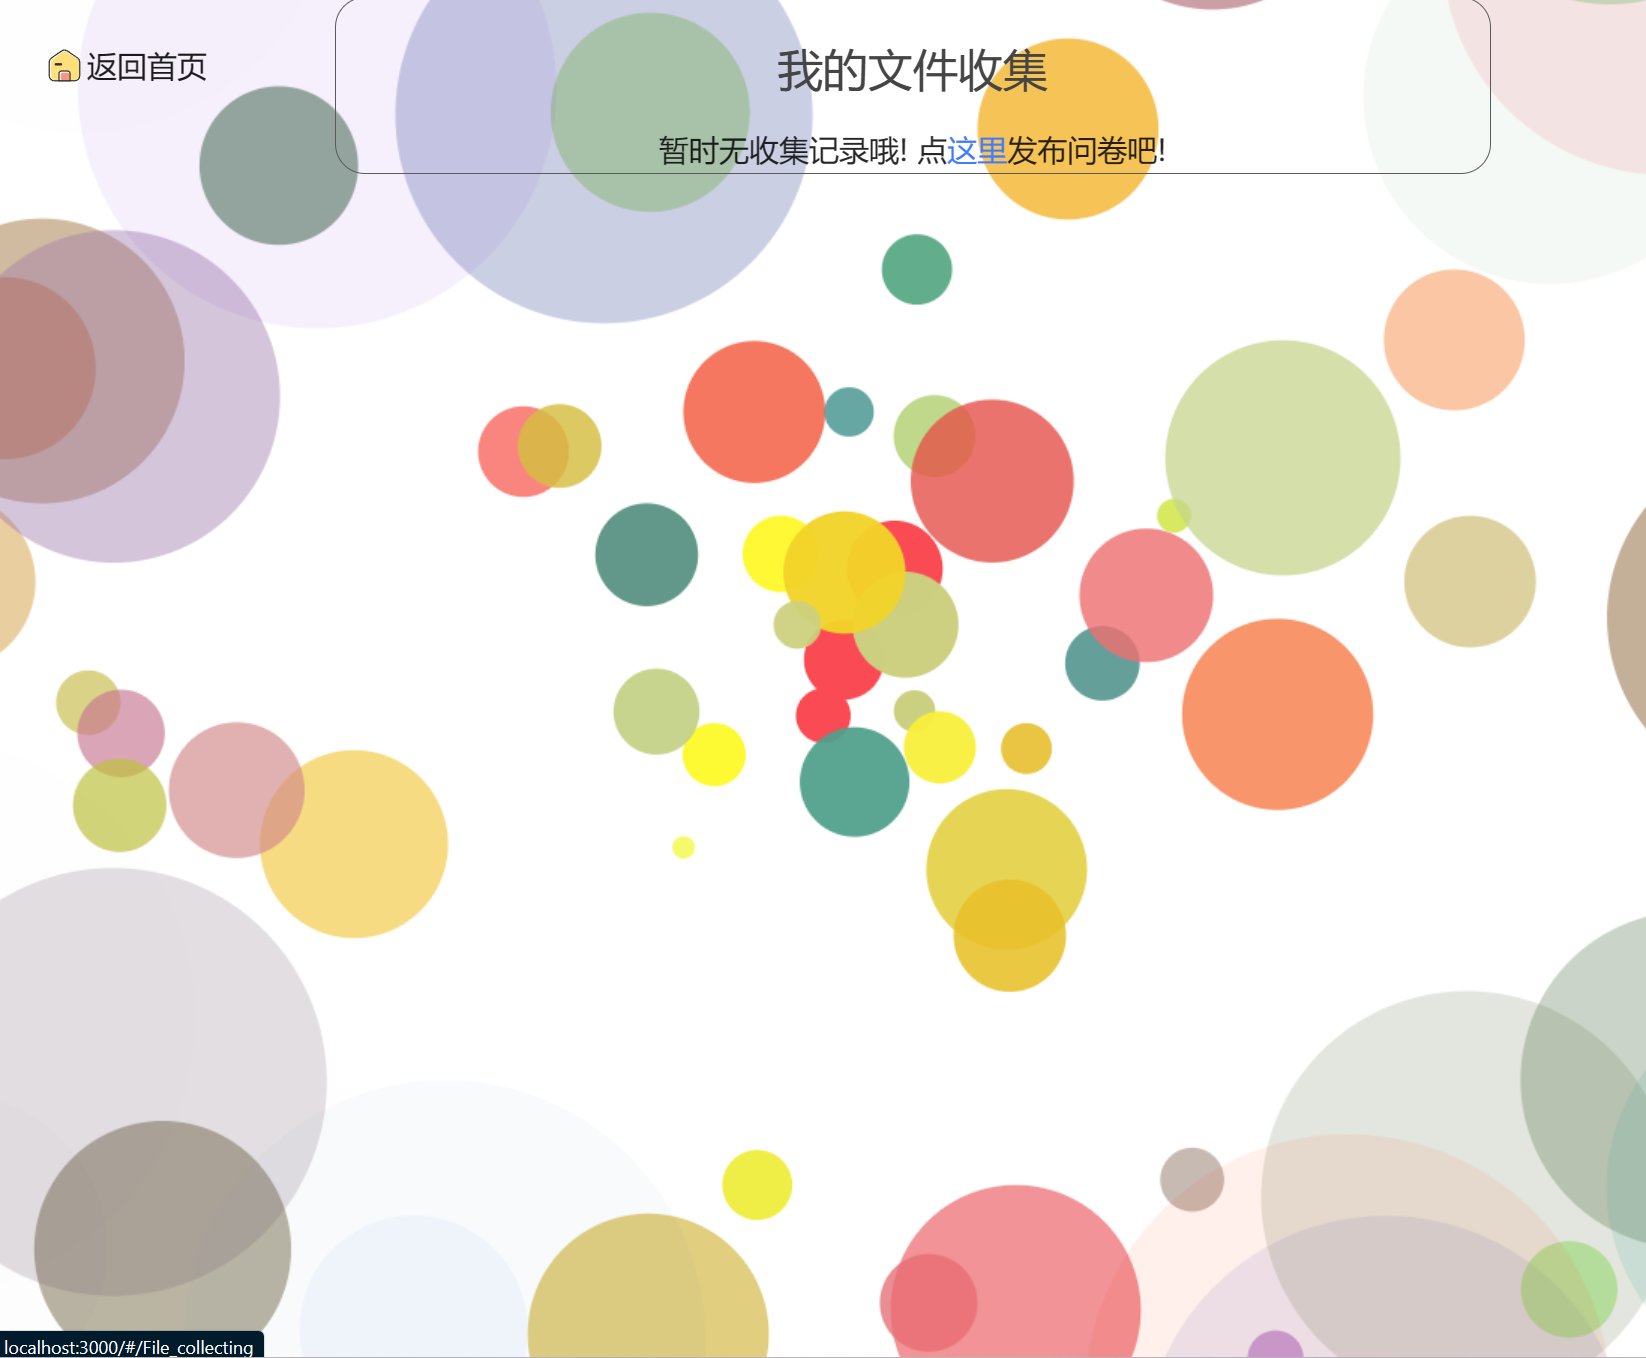
\includegraphics[width=0.9\textwidth]{收集记录.png}
	\end{figure}
	
	每个收集都有5种操作按钮:“分享”、“统计”、“编辑”(已截止为“重启”)、复制、停止(已截止为“删除”)。点击\hlc{统计}按钮可以进入对应收集的“收集详情”页面。
	
	“收集详情”页面有三种显示模式:应交名单、提交记录、统计图表。
	\begin{itemize}
		\item 应交名单界面,可以添加当前收集的应交者名单,系统自动生成 .csv 文件
		\item 提交记录界面,可以查看所有提交信息的时间、提交者等
		\item 统计图表界面,可以查看选择题、问卷题的统计情况
	\end{itemize}
	\item{\bf 修改收集}\\
	如果需要修改已创建的收集,可以在收集详情界面点击\hlc{编辑}按钮,进入编辑状态。处于编辑状态时,可以修改收集标题、收集者、截止时间、详情描述,以及题目的具体内容,但不能删除、添加题目或调换题目的位置。编辑完毕后,点击最下方的\hlc{编辑完成}按钮即可提交编辑,完成修改。\\
	{\bf Note:修改收集不会影响已收问卷。}
	\item{\bf 复制收集}\\
	如果需要新建和已创建的收集结构相同或类似的收集,可以在收集详情界面点击\hlc{复制}按钮,系统会按照对应的收集创建一个结构完全相同的收集,您可以在此基础上进行修改。编辑完毕后,点击最下方的\hlc{创建}按钮即可创建收集。\\
	{\bf Note:复制收集不会影响被复制收集,原有收集的文件不会被复制到新的收集中。}
	\item {\bf  到期提醒}\\
	创建收集之后,您还可以开启到期提醒功能,系统将通过邮件提醒应交名单中尚未提交的提交者尽快提交。
	\item {\bf 统计汇总}\\
	对于添加了应交名单的收集,系统会自动记录已提交和未提交的名单,生成 Excel 表格,点击\hlc{ 查看汇总}即可下载。
	\item {\bf 个人信息}\\
	您可以通过点击左上角您的用户名进入到个人信息界面,并且自行进行修改。
			\begin{figure}[!htb]
		\centering
		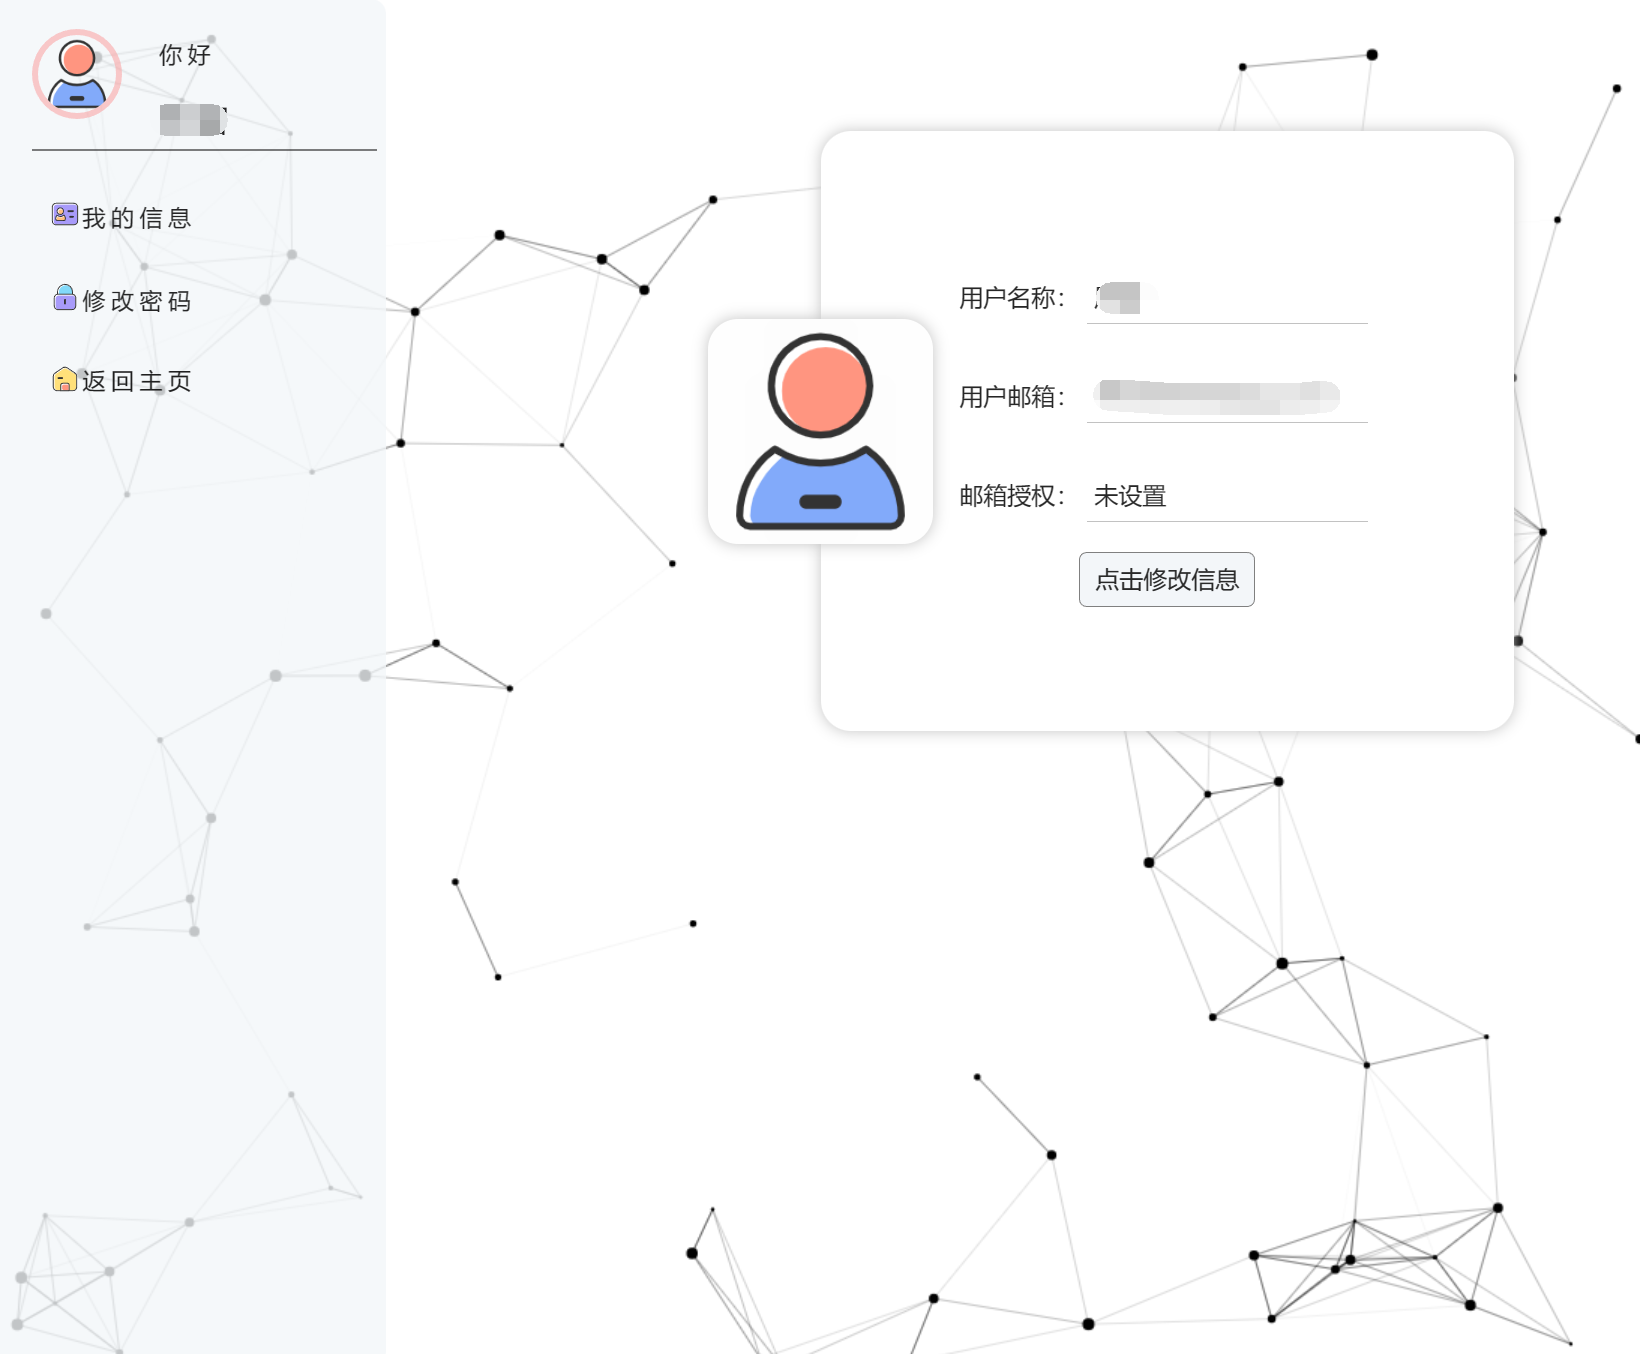
\includegraphics[width=0.9\textwidth]{个人信息.png}
	\end{figure}
\end{itemize}

\subsection{提交者}
\begin{itemize}
	\item \textbf{加入收集}\\
	提交者点击收集者发布的收集链接(或扫描对应收集的二维码),进入填写界面。如果提交者已注册并填写了邮箱信息,在登录状态下提交收集时,默认启用到期提醒功能。\\
	\textbf{Info:到期提醒功能是指在截止日期前 X 小时,若提交者位于收集者设置的应交名单中,系统将通过邮件方式提醒尚未提交的人员尽快提交。}
	\item \textbf{填写信息}\\
	收集问卷中可能包含以下几种类型的题目:填空题、选择题、文件题和问卷题。
	\begin{enumerate}
		\item \textbf{填空题}:例如姓名、学号、班级等。在输入框中填入相应信息即可。
		\item \textbf{选择题}:选择题分为单选题和多选题。
		\begin{itemize}
			\item \textbf{单选题}:
			选择您认为最合适的一个选项,点击选项前的圆形框即可选择。如需修改答案,直接点击修改后选项前的圆形框即可。
			\item \textbf{多选题}:
			选择您认为合适的多个选项,点击选项前的方形框即可选择,再次点击可取消选择。
		\end{itemize}
		\item \textbf{文件题}:点击\hlc{选择文件}按钮,从本地选择要上传的文件。
		\item \textbf{问卷题}:与选择题类似,选择您认为合适的一个或多个选项,点击选项前的选项框即可选择。如为多选题,再次点击选项框即可取消选择。
	\end{enumerate}
	\item \textbf{提交收集}\\
	填写完毕后,点击最下方的\hlc{提交}按钮,完成问卷提交。在截止日期前,您可以进行多次提交。
	
	\textbf{Note:提交成功后,您将会看到提交成功的页面。}
	
	\item \textbf{到期提醒}\\
	在截止日期前 X 小时,收集者将通过邮箱向尚未提交收集的待提交者发送催交邮件。
\end{itemize}
\clearpage
\section{常见问题}

\subsection{收集者}

\subsubsection*{1.1 发布收集后,提交者能看到我管理的其他文件吗?}

不能,仅\textbf{您本人}能够查看您所属目录下的文件。

\subsubsection*{1.2 有些提交者提交了不止一次,如何保证收集文件正确性?}

如果提交者后一次提交的文件格式(如后缀名为 .pdf)与前一次{\bf 完全相同},则后一次提交的文件会覆盖前一次提交的文件;如果不同,则会生成一个按照重命名规则命名的文件夹,里面存放提交者提交的\textbf{所有}文件。

\begin{example}
	文件覆盖:
	
	有一位提交者{华小科}第一次提交了名为“计算机网络第一次作业.docx”的文件,在截止日期前发现有错误需要修改,于是再次提交了修改后的文件,名称仍为“计算机网络第一次作业.docx”。这种情况下,后一次提交的文件会覆盖前一次的文件,系统中最后保留的是后一次提交的文件。
若华小科后一次提交的文件名称为“计算机网络第一次作业.doc”,尽管两次提交的文件名称相同,由于后缀名不同(第一次是 .docx,第二次是 .doc),系统会建立一个名为“计算机网络第一次作业”的目录,将两次提交的文件都保存在其中,最终形成如下目录结构:


\begin{lstlisting}
	|-- 计算机网络第一次作业/
	|   |-- 计算机网络第一次作业.doc
	|   |-- 计算机网络第一次作业.docx
\end{lstlisting}

\end{example}

\subsubsection*{1.3 如何获取收集的统计信息?}


{\bf Tips:查看汇总按钮在收集详情页面右侧}。

在收集截止后,系统将在您对应收集的文件夹中生成一个 Excel 表格,记录收集的相关信息。您可以在收集详情页面点击“查看汇总”按钮下载该 Excel 表格。

\subsubsection*{1.4 如何将收集到的文件保存到本地?}


{\bf Tips:下载文件按钮在收集详情页面右侧。}


您可以在收集详情页面点击“下载文件”按钮手动获取当前收集到的所有文件的压缩包;在收集截止后,系统会依据您注册的邮箱信息,自动将对应的收集以 zip 压缩包的形式通过邮件发送到您的邮箱。

\subsection{提交者}

\subsubsection*{2.1 文件需要命名后再上传吗?}
如果收集者设置了重命名规则,系统会根据您填写的提交信息自动重命名提交文件,您无需在意文件的命名。

\subsubsection*{2.2 提交了错误的文件怎么办?}

重新提交正确的文件,并填写完全相同的提交信息即可。收件箱系统将智能合并提交信息完全一致的文件。

\subsubsection*{2.3 提交信息填写错误怎么办?}

您可以在收集截止前,填写正确的提交信息再次提交。

\subsubsection*{2.4 其他人能看到我提交的文件吗?}

只有收集任务的发布者和您本人有权限查看您提交的文件,请放心提交。




\end{document}
